The user will be presented with a simple and easy to use interface, which
assumes and requires no knowledge of security. The most complicated thing that
the user will have to do is transmit to other users their public key. We plan
to alleviate this process by encoding the public key as both a QR code and
plaintext string (depending on user preference), both of which may be easily
transmitted via email, SMS, meeting in person, or over any other channel.

Upon connecting to the system for the first time, the user will be prompted to
enter a username, and any profile information they choose to share, and a
passphrase. They will be urged to avoid using their real name as their username,
and informed that profile information is shared on a case by case basis, and is
not automatically visible to people whom they add. The entered passphrase will
be used to deterministically derive an AES key which will be used to encrypt the
users keypair and local DB. The user will be given the option of creating a
second passphrase which, when entered, will overwrite the keypair and local DB
with random data.

They will then be brought to the main page of the system, where they (and)
people they authorize, may post message. There will be a prompt for them to add
peoples public keys, and the option to add either a QR encoded or plaintext
encoded public key.

Upon adding another's public key, they will first be informed of that persons
username, and prompted to categorise the person. The user will be able to create
a number of categories into which they can place that user. Already created
categories will be displayed. One person may be added to multiple categories,
and nobody but the user is aware that this occurs. Depending upon the categories
the person is entered into, that person gains the ability to view certain
content posted by the user.

When the user posts a message they are prompted to enter a recipient, this may
be: a previously created category (such as friend, co-worker); a number
of individuals; or any combination thereof.

Upon receiving a message a sound is played and the user is informed. They are
then able to click on the notification to open the message, and chat. When
chatting with another user they have the ability to 'ignore' that user, in this
case the user will see no more messages from that user.

\section{System Boundary Diagram}
We can see the users interaction with the system below in the System Boundary 
Diagram:

\begin{figure}[h]
    \centering
    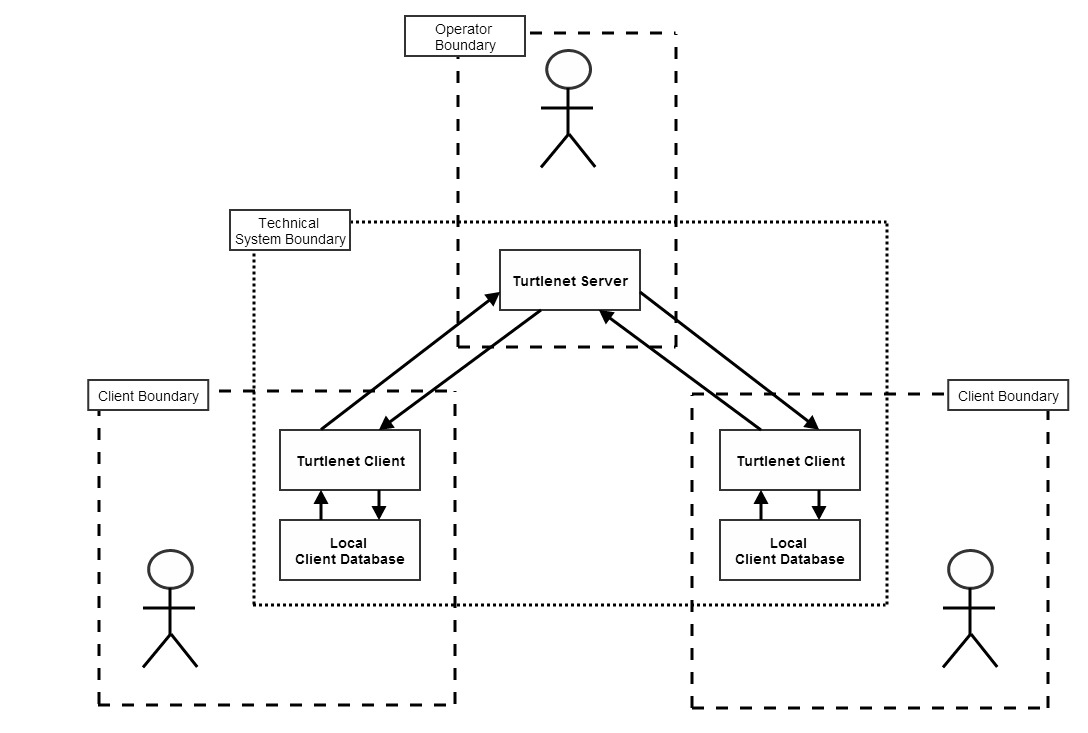
\includegraphics[width=\textwidth]{images/requirements/systemboundarydiagram.jpg}
    \caption{System Boundary Diagram}
    \label{fig:sbd_diag}
\end{figure}

Each client (of which there may be many) has his own client boundary consisting 
of his database and program client, whilst the server operators have their own 
boundary consisting of just the server. You can see in the diagram that at no 
point does the server operator or user functionality coincide with each other, 
leaving their privacy fully independent of one another. Each client (of which 
there may be many) has his own client boundary consisting of his database and 
program client, whilst the server operators have their own boundary consisting 
of just the server.